\documentclass{article}
\usepackage{latexsym,amsmath,amssymb,tabu,CJKutf8,graphicx,bm,blkarray,delarray,float}
\textheight 9in \textwidth 6.5in \oddsidemargin 0pt \topmargin -8pt
\pagestyle{plain}

\usepackage[colorlinks,linkcolor=blue]{hyperref}


\newcommand{\phit}{\phi_{t+\Delta t}}
\begin{document}
\begin{CJK}{UTF8}{gkai}
 

\title{Broadly Accessible Self-Consistent Field Theory for Block Polymer Materials Discovery\\
(广泛适用于嵌段聚合物物质发现的自洽场理论)}
\author{Akash Arora, Jian Qin, David C. Morse,Kris T. Delaney,Glenn H. Fredrickson, Frank S. Bates, and Kevin D. Dorfman}
\date{2016}
\maketitle
\begin{quotation}
\textbf{摘要}
自洽场理论(SCFT)是一个设计和解释嵌段聚合物材料实验有用的工具。在这个角度,我们通过两种方法降低了实验组使用SCFT的门槛。首先,我们提出了一个改进版的开源聚合物自洽场(PSCF)软件包和基础理论教学介绍。其次,我们对于SCFT中计算需要的初始猜测的方法进行了讨论。为了展示我们的方法,我们提出了两个案例研究,其中一个是用电脑来模拟(1)体心立方结构、面心立方结构、A15、两嵌段聚合物溶体的Frank-Kasper$~\sigma$球型相(2)ABAC四嵌段三元共聚物的核-壳形态。

\section{介绍}
SCFT是研究块状聚合物相行为的最强大的工具之一。经验表明,SCFT很擅长预测有序相的相对稳定性和有序-有序转变的位置,但SCFT对嵌段共聚物熔体有序-无序的转变的预测并不准确,但这些不精准的预测为理解和预测体系结构中的相似链系之间的趋势提供了一个有用的起点。

很多人认为平时问题在于理论本身复杂性,其实是在理论的实际实施方面有两个关键问题。

第一个问题是,还没有健全(免费)的软件去实现所需的数值方法。

第二个问题是,作为对SCFT计算输入的初始猜测的生成,特别是对于复杂的相。SCFT是由一组高度非线性的方程组控制,通常有多个可能的解。

SCF方程一般采用迭代法求解,可以从不同的初始猜测收敛到不同的解,或者根本不收敛。为了利用SCFT来研究特定的结构或相位,或者比较竞争结构的自由能,人们必须知道如何产生将收敛到特定的结构的初始猜测。
对于软件问题的解决,本文介绍了由Morse及同事开发的\underline{开源聚合物自洽场(PSCF)}代码
(\url{http://research.cems.umn.edu/morse/code/pscf/home.php.})
我们还提供了标准磁盘映像\\
(dmg文件)(\url{http://pscf.cems.umn.edu})和Linux二进制可执行文件的形式,为当前版本的OSX提供对二进制安装程序的访问。我们还提供了各种非传统的材料供公众下载。具体来说,除了源代码提供的输入文件和解决方案的集合之外,我们还为本文中的所有示例提供了\href{http://pubs.acs.org/doi/suppl/10.1021/acs.macromol.6b00107/suppl_file/ma6b00107_si_001.pdf}{Supporting Information},并详细描述了它们在Web站点(\url{http://pscf.cems.umn.edu.})上的生成和实现。最后,我们对代码做了一些改进,其中最重要的是Anderson混合迭代算法的实现。新算法允许PSCF去计算所需要的大型单元的复杂相位,如Frank-Kasper$~\sigma$相。

为了消除初始化路障,为生成SCFT的输入所需的的初始猜测我们提供了两种方法:第一种方法适合于含有离散物体(例如球体或圆柱体)的结构,方法基于傅里叶空间形状因子的计算,就像分析这些相位的散射时所做的那样。第二种更适合于网络相,是基于一种水平集方法。每个示例的详细信息都嵌入到Matlab脚本中(见\href{http://pubs.acs.org/doi/suppl/10.1021/acs.macromol.6b00107/suppl_file/ma6b00107_si_001.pdf}{Supporting Information}S3和S6两部分),这些脚本可以用于生成输入文件。我们用来生成初始场的Matlab脚本可以使用Matlab或它的开放源代码相关器来执行,但是我们的可视化脚本使用的是一些仅在Matlab中可用的函数。

论文大概内容是,第二节描述了SCFT方法。第三节讨论了粒子相(particle phases)和网络相(network phases)产生初始场猜测的策略。第四节介绍了上述粒子相案例研究的结果。第五节最后提出了进一步改进的一些展望。

\section{SCFT在PSCF中的实现}
\textbf{2.1.自洽场方程.}\\
PSCF程序用于求解不可压缩聚合物液体形成的空间周期结构的SCFT方程。一般情况下,该体系可以包含任意数量的线性嵌段共聚物、均聚物和小分子溶剂的混合物。为了简化讨论,我们给出了单一成分嵌段共聚物熔体的相应方程,并在\href{http://pubs.acs.org/doi/suppl/10.1021/acs.macromol.6b00107/suppl_file/ma6b00107_si_001.pdf}{Supporting Information}S10部分讨论了含溶剂混合物的相应方程。

我们考虑一种具有$N$个单体和$B$个嵌段的线性多嵌段共聚物的熔体,且具有$C$类不同类型的单体。用路径变量$s$,$0<s<N$标记特定单体,用$\alpha=1,...,C$标记不同类型的单体。在SCFT中,链的构型通常用随机游走统计量来模拟,而单体-单体相互作用则被自洽化学势场相互作用所取代。在下面,$\omega_{\alpha}(\mathbf{r})$表示作用于位置$\mathbf{r}$处的$\alpha$型单体的一个有效的化学势场,它是由链之间的相互作用而产生的。SCFT公式是基于对化学势场中随机游动聚合物的统计性质的计算,其中不同类型的单体被这些化学势场吸引到不同的空间区域。这样的随机游动所需的统计性质可以用下列一对修正的扩散方程(MDEs)的解来描述
\begin{equation}\label{1}
\begin{aligned}
\frac{\partial q(\mathbf{r},s)}{\partial s} & = \left[ \frac{b_{\alpha (s)}}{6}\nabla ^2 - \omega_{\alpha (s)}(\mathbf{r}) \right]q(\mathbf{r},s)\\
-\frac{\partial q^{+}(\mathbf{r},s)}{\partial s} & = \left[ \frac{b_{\alpha (s)}}{6}\nabla ^2 - \omega_{\alpha (s)}(\mathbf{r}) \right]q^{+}(\mathbf{r},s)\\
\end{aligned}
\end{equation}
两个“传播子”函数$q(\mathbf{r},s)$和$q^{+}(\mathbf{r},s)$具有初始条件
\begin{equation}\label{2}
q(\mathbf{r},0)=q^{+}(\mathbf{r},N)=1
\end{equation}
其中,$b_{\alpha (s)}$是$\alpha (s)$型单体的统计段长,$\omega_{\alpha (s)}$是相应的单体化学势场,$\alpha (s)$是含单体$s$的单体类型指数。函数$q(\mathbf{r},s)$是从单体$0$开始,被约束具有特定位置$\mathbf{r}$时单体$s$的链段的统计权重(即规范的,约束的配分函数)。数量$q^{+}(\mathbf{r},s)$是一个互补传播子,它给出了剩余链段的统计权重,从单体$N$开始,到位置$\mathbf{r}$结束。

在这里,我们考虑一个不可压缩的熔体,其中每个单体都占据体积$v$,因此每链的体积是$Nv$。

以$v=1$(即反单体体积单位(units of inverse monomer volume))为单位,给出了$\alpha$型在$\mathbf{r}$位置的密度$\phi_{\alpha}(\mathbf{r})$
\begin{equation}\label{3}
\phi_{\alpha}(\mathbf{r})=\frac{1}{NQ}\int _{\alpha}~q(\mathbf{r},s)q^{+}(\mathbf{r},s) \mathrm{d}s
\end{equation}
其中
\begin{equation}\label{4}
Q=\frac{1}{V}\int ~q(\mathbf{r},N) \mathrm{d}\mathbf{r}
\end{equation}
是一个无约束链的配分函数,其中关于$\mathbf{r}$的积分取在一个周期结构的单位-细胞上,$V$是单位-细胞体积。不可压缩性的约束在这些单位中表示为下列条件:
\begin{equation}\label{5}
\sum _{\alpha}\phi_{\alpha}(\mathbf{r})=1
\end{equation}
当满足此约束时,$\phi_{\alpha}(\mathbf{r})$可以解释为$\alpha$类型在$\mathbf{r}$位置的局部体积分数。

化学势场$\omega_{\alpha (s)}(\mathbf{r})$是以不可压缩液体自洽场的标准形式给出的
\begin{equation}\label{6}
\omega_{\alpha (s)}(\mathbf{r})=\sum _{\beta \neq \alpha} \chi_{\alpha \beta}\phi_{\beta}(\mathbf{r})+\xi(\mathbf{r})
\end{equation}
其中$\chi_{\alpha\beta}$是$\alpha$和$\beta$类单体相互作用的二重Flory-Huggins相互作用参数,且$\chi_{\alpha \alpha}=0$。$\xi(\mathbf{r})$是满足约束条件所必须选择的拉格朗日乘因子。

方程(\ref{1})-(\ref{6})代表了SCFT一组完整的方程,需要数值求解才能得到化学势场$\omega_{\alpha(s)}$和相应的体积分数$\phi_{\alpha}(\mathbf{r})$的解。注意方程的耦合性质:公式(\ref{6})中的势场$\omega_{\alpha(s)}$取决于单体浓度$\phi(\mathbf{r})$,这进一步依赖于公式(\ref{3})中的传播子$q(\mathbf{r},s)$和$q^{+}(\mathbf{r},s)$的乘积。然而,公式(\ref{1})依赖于$\omega_{\alpha (s)}$。因此,在已知体积分数之前,势场是无法计算的,而在不知道势场的情况下,不能知道体积分数。结果表明,方程(\ref{1})−(\ref{6})在$\omega_{\alpha (s)}$中形成了一组非线性方程组,只能用迭代方法求解。
\begin{figure}[H]
	\centering
	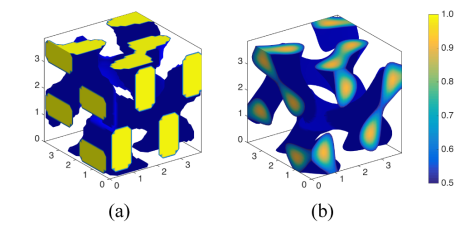
\includegraphics[scale=0.5]{./figures/22.png}
	\caption{SCFT求解所涉及的步骤的流程图。蓝色框表示在PSCF中实现的过程,而红色框表示为$\omega$场生成合理的初始猜测所需的过程。}
	\label{figure1}
\end{figure}
图\ref{figure21}给出了用于求解SCFT方程的迭代数值算法。蓝色框表示SCFT主算法。主要算法以化学势场$\omega_{\alpha (s)}$的初值为输入。初始场的选择对算法收敛性的判定有着至关重要的作用,并在下一节中对其进行了详细的讨论。利用这些初始势场,求解出MDEs(方程(\ref{1})),得到$q(\mathbf{r},s)$和$q^{+}(\mathbf{r},s)$。然后通过公式(\ref{3})和(\ref{4})沿链轮廓积分单体体积分数来计算单体体积分数。计算了体积分数后,计算了自洽场方程(\ref{6})和条件(\ref{5})中的误差。如果这些误差大于某些指定的容限$\epsilon$,则使用迭代格式更新化学势场,如牛顿法、Anderson混合法、或semi-implicit Seidel方法。然后使用更新的势场作为输入,整个过程被重复,直到(\ref{5})和(\ref{6})中的误差降到指定的容限以下。

一旦得到了(\ref{1})-(\ref{6})的解,得到的结构的每个单体的自由能计算如下:
\begin{equation}\label{7}
\begin{aligned}
\frac{F}{k_BT}\frac{v}{V} & =  -\frac{1}{N}\ln (eQ)+\frac{1}{2V}\sum _{\alpha \beta} \chi_{\alpha \beta}\int \phi_{\alpha}(\mathbf{r})\phi_{\beta}(\mathbf{r}) \mathrm{d}\mathbf{r}\\
& - \frac{1}{V}\sum _{\alpha} \int \omega_{\alpha}(\mathbf{r})\phi_{\alpha}(\mathbf{r})\mathrm{d}\mathbf{r}\\
\end{aligned}
\end{equation}
不同的自洽解对应于不同的中间相;每个可能的空间周期解代表有序结构,而齐次解对应于无序相。

空间周期的中间相的自由能一般取决于晶胞的尺寸和(对某些单位胞系)晶体轴间的角度。平衡自由能是由单元给出的,它是公式(\ref{7})中给出的最小化自由能。因此,计算给定相位的平衡自由能需要优化单元参数和求解SCF方程。对于层状、六角形或立方相的简单情况,这相当于对单个单元尺寸的值进行优化。对于更复杂的单元,例如正交Fddd相位,这可能需要对几个单元参数进行多维优化。优化单元的复杂算法可以利用SCFT自由能的导数有关单元参数的知识,这些知识可以作为修正扩散方程解的一部分,并以最小的附加费用计算。PSCF可以选择在更新势场的同时更新单元参数。

为了利用SCFT单元的计算来构造相图,通过比较一组相互竞争的中间相的自由能,利用每个候选相的最佳单元参数,来确定参数空间中各点的热力学稳定相。这一程序中固有的不确定因素是需要事先构造一组可能的候选结构,并且不可能确定所提议的名单是否包括全局最小值。

图\ref{figure21}所示的流程图几乎可以描述任何SCFT的实现。不同的研究人员和研究小组所提出的实现方法之间最大的区别是,对于固定化学势场,求解MDEs的的数值算法的选择(这是该算法的循环)、更新化学势场的迭代算法的选择和(在某些情况下)晶体单元参数的选择是不同的。
%对于单元计算开发的代码也不同,无论它们在解决方案上强加特定的空间群对称。

本节的剩余部分简要描述了由PSCF提供的算法和特征。\\
\textbf{2.2.MDE Solver.}\\
在PSCF码中,MDEs采用Rasmussen和Kalosakas提出的拟谱方法的一个变形来求解。在PSCF中,同样的算法可以用来描述完全三维的周期性结构(如共连续网络或球体形成相),二维周期结构(如六角形柱状相)或一维层状相。在拟谱方法中,将单个1-、2-或3维单元内的MDES的周期在规则的维网格上离散化。通过对具有小时间步长$\Delta s$的方程进行“时间步进”,对类似时间的轮廓变量$s$也进行离散化。一个典型的当代计算可能是沿每个空间方向使用32到128个网格点和每一条链用100个路径段进行分割。

拟谱算法的特点是利用快速傅里叶变换(FFT)在周期域中准确有效地表示$q$和$q^{+}$(参见公式\ref{1})的拉普拉斯算子。所需的初始拟谱算法要求一个前向FFT和一个逆FFT的计算等高线长度时间步长为$\Delta s$,并给出了$(\Delta s)^2$的全局精度。

我们PSCF的实现版本依赖于FFTW软件包(\url{http://www.fftw.org/})来计算所需的转换。相应的OSX应用程序(\url{http://pscf.cems.umn.edu})也可供公众下载,所有必要库已经嵌入到应用程序中,只需双击图标即可运行。

在MDE求解中使用FFTs的一个好处是,无论是在实空间中,作为在实空间网格节点处的一组值,还是在傅里叶空间中,作为离散傅里叶变换的系数,PSCF源代码提供了对化学势和单体浓度场表示的现成访问。在实空间网格表示中,三维势场$\omega (\mathbf{r})$在网格点$\mathbf{r}(m_1,m_2,m_3)$给出,其中$m_i \in \left[ 0,N_i-1 \right]$
\begin{equation}\label{8}
\mathbf{r}(m_1,m_2,m_3)=\sum _{i=1}^{3}\mathbf{a}_i \frac{m_i}{N_i}
\end{equation}
其中,$N_i$是向$i$方向的网格点数。这里,$\mathbf{a}_1,\mathbf{a}_2$和$\mathbf{a}_3$是标准常规单元的Bravais lattice向量,
%例如立方单元,用于具有立方对称性的相位。
傅里叶空间表示是一个平面波基函数的展开式,它由reciprocal lattice 向量给出,
\begin{equation}\label{9}
\mathbf{q}(n_1,n_2,n_3)=\sum _{i=1}^{3}n_i\mathbf{b}_i
\end{equation}
整数$n_i\in[0,N_i-1]$的范围内,$\mathbf{b}_1,\mathbf{b}_2$和$\mathbf{b}_3$是满足$\mathbf{a}_i \cdot \mathbf{b}_j=2\pi \delta _{ij}$的reciprocal lattice basis vectors向量。\\
\textbf{2.3.Symmetry.}拟谱MDE求解使用的空间离散化施加周期边界条件,但不施加任何空间群对称性,反射平面、离散旋转对称或滑动平面或包括由一部分的平移引起的平移的螺杆轴对称单元。然而,PSCF所使用的外部迭代算法和用于输入和输出化学势和浓度场的文件格式都使用更为紧凑的表示特定空间群对称性的场作为对称适配(symmetry-adapted)傅里叶展开。PSCF的用户可能需要对这种扩展有一定的了解,因为它是PSCF用于输入和输出单体化学势和浓度场的文件格式的基础,因此我们在这里提供了一个比较详细的技术描述。

在symmetry-adapted傅里叶展开中,已知空间群对称性的实周期场$\omega (\mathbf{r})$被展开为和
\begin{equation}\label{10}
\omega (\mathbf{r})=\sum _{n=1}^{P} a_nf_n(\mathbf{r})
\end{equation}

$P$个symmetry-adapted基函数$f_1(\mathbf{r}),...,f_P(\mathbf{r})$和实系数$a_i,...,a_P$。每个symmetry-adapted基函数都是特征值问题$-\Delta ^2f_i(\mathbf{r})=\lambda _if_i(\mathbf{r})$的实周期解,它在特定空间群的所有对称元下都是不变的。

作为一个简单的例子,考虑一维周期为$L$的且具有反对称性$\omega(x)=\omega(-x)$周期场$\omega (x)$。可以用symmetry-adapted基函数$f_1(x)=1$和$f_n(x)=\sqrt{2}\cos\left[ 2\pi (n-1)x/L \right]$展开,$n=2,3,...,P$。一般实一维周期函数不具有反对称性的展开式将使用包含余弦基函数和正弦基函数的展开式。

一般情况下,任意$1,2$或$3$维空间群的每个symmetry-adapted基函数$f_n(\mathbf{r})$都可以表示为和
\begin{equation}\label{11}
f_n(\mathbf{r})=\frac{1}{\sqrt{S}}\sum_{j=1}^{S}c_je^{i\mathbf{q}_j\cdot \mathbf{r}}
\end{equation}
具有一组S平面波的reciprocal lattice 波向量$\mathbf{q}_1,...,\mathbf{q}_s$,它们通过空间群相互关联。每个这种对称相关的波向量集有时被称为“star”。例如,立方晶体中reciprocal lattice向量的每个星对应于向量$\mathbf{q}(h,k,l)$,它们之间通过排列和整数$h,k$和$l$符号的变化而相互关联。symmetry-adapted基函数的展开式只包含与star相关的基函数,其中包含波矢这是由所选空间群的系统规则所允许的。例如,对于BCC晶体的展开不包含$h+k+l$是奇数相关联的基函数。

方程\ref{11}中的系数$c_1,...,c_{n_s}$通常是复数,且$\left|c_j\right|=1$。对于反对称空间群$\omega(\mathbf{r})=\omega(\mathbf{-r})$,这些系数都可以看作实数,$c_j=\pm 1$。然而,在某些近似群中,星体内不同平面波的系数可以有$\pm 1$的相反符号值。例如,这发生在阶段(gyroid phase)的̅$I\alpha \bar{3} d$组中。

PSCF的迭代算法和输入输出场的文件格式都采用对称傅里叶展开来表示所有化学势场和单体浓度场。$\omega$势场的初始读取和输出$\omega$和$\phi$场的解决方案所使用的文件格式包含每个场的这些系数的列表,方程(\ref{10})中给出了一个形式的扩展。迭代算法通过修改此展开中的系数来更新$\omega$势场后MDEs的每一个解。在从文件中读取$\omega$势场的初始猜测之后,每次更新这些场之后,该表示都会在解MDE解之前自动转换为通用的使用MDEs解Fourier展开。在求解和计算单体浓度场后,将生成的浓度场转换回symmetry-adapted表示,供外部迭代算法使用并输出到文件中。在外迭代循环中使用symmetry-adapted展开,自动限制了对具有特定空间群对称性的SCF方程解的搜索。

用户在输入脚本中输入所需空间组的名称,该脚本还包含FFT网格的每个方向上的网格点数。在读取这部分输入脚本之后,在读取$\omega$势场的初始猜测之前,PSCF自动生成一组适合于指定空间组和FFT网格的symmetry-adapted基函数。对于为特定空间组和网格生成的基础的描述,可以通过调用输出输入脚本中的Output-Wave命令将其输出到文本文件中。PSCF可以读取和正确解释为具有相同空间组但具有不同空间的结构而生成的$\omega$势场,以便将粗网格的模拟用作细网格计算的输入。PSCF还提供了输入脚本命令,允许用户在包含$\omega$或$\phi$场对称适应表示的文件和在实空间网格节点上包含这些字段值的文件之间进行转换,方法是读取这两种格式中的一种格式的文件,并在另一种格式中输出的文件。有关这些特性和其他特性的更详细说明,请参见Web用户手册\url{http://research.cems.umn.edu/morse/code/pscf/home.php.}。

虽然PSCF主要用于单元计算,并具有强加的空间组对称性,但用户可以通过指定标识空间组(由空间组标签“i”标识)来禁用此限制。这个平凡的空间群除了空间周期性外没有对称性,并相应地使PSCF产生一个完整的正弦波和余弦波基。\\
\textbf{2.4.迭代算法}PSCF允许用户选择两个不同的迭代算法来更新$\omega$势场和(任意的)优化单元尺寸。第一种算法是拟牛顿法(NR),其首次发布以来一直是PSCF的一部分。本文实现的第二种算法是一种Jacobian-free Anderson-mixing algorithm。

在PSCF中实现的拟牛顿方法结合了Jacobian矩阵的物理初始逼近和Broyden方法来更新近似Jacobian和一个backtracking line  search(回溯线搜索)。该算法既可用于求解固定单元中SCF方程或者同时求解SCF方程,并在每次迭代时使用$\omega$势场和单元尺寸的完全耦合同时更新,找到最佳的单元尺寸。该算法的初始逼近是用数值差分法构造的,用来计算表示误差导数(残差向量的分量)的矩阵中相对于$\omega$场的小分量系数的部分,而对于较高分量的导数则使用简单的RPA逼近法。该算法要求用户输入一个名为Ncut的截止点,以指定需要计算数值导数的symmetry-adapted傅里叶分量的数目。

这个拟牛顿/Broyden算法的性能和成本的几个方面需要被用户了解。构造Jacobian的初始近似是一个潜在的缓慢过程,其计算成本随着截止Ncut的选择而近似线性上升。因此,该算法的用户应该对该参数的选择进行实验,以确定需要多大的值才能获得收敛性。我们通常选择Ncut=100−200。该算法在构造初始节点后,往往需要几十步,最后几步几乎是二次收敛。该算法的一个优点是优化单元的成本低;寻找最优单元所需的步骤数一般可与在固定单元中求解SCF方程所需的步骤数相比较。该算法的一个重要限制是存储近似Jacobian矩阵所需的大量内存,它与计算中使用的对称自适应基函数的平方成正比。对于需要$10^4$个以上基函数的计算,无论是因为结构是强的,还是因为它有一个复杂的单元(如Frank−Kasper $\sigma$相),所需内存可能超过当前典型硬件上可用的内存。

我们最近增加了Anderson混合算法到PSCF中,主要是由于需要一种比拟牛顿格式更小的内存需求的迭代算法。Anderson混合格式所需的内存仅随symmetry-adapted基函数的数目线性增加,通常比存储非均匀解所需的内存少得多。

这里需要实现Anderson混合算法来模拟单CPU核上的Frank−Kasper $\sigma$相。在我们的经验中,用于求解固定单元中的方程的Anderson混合算法通常比准牛顿算法需要更多的步骤,且每步平均计算成本较低。我们目前这种算法的一个缺点是,用一个最优单元计算一个解所需的时间远远大于在固定单元中求解该方程所需的时间。

PSCF中的拟牛顿和Anderson混合算法都不是绝对稳定的,也不能保证算法收敛到$\omega$势场的任意初始猜测。这两种算法从良好的初始猜测中相对较快地收敛,但是,它的稳健型不如一些可以收敛到解的方案(尽管不一定是所需的解)甚至是从随机的初始$\omega$势场。未来关于迭代算法的研究将集中在提供更稳健的迭代算法作为替代,以及改进在拟牛顿格式以外的算法中用于优化单元格的方法。

介绍了PSCF中提供的许多特征,以简化相图的计算。在这类计算中,可以通过求解两个或多个候选相在参数空间中沿一条直线排列的参数点的序列上的近似问题,和确定竞争相的自由能在哪里的变化符号差异来识别相边界。PSCF提供了一个用户命令(SWEEP要求),该命令允许用户使用解决方案的二阶连续完成这样的计算序列,从而使除第一个或第二个参数点之外的所有参数点都快速收敛。在这样的计算序列中使用PSCF拟牛顿算法是特别有效的,因为该特征的实现尽可能地重用了以前的计算中获得的近似 Jacobian 。这种延续特性还使用户可以相对容易地从以前获得的特定结构的解决方案(有时可以从随代码分发的示例中获得)开始,在不同的参数集中获得相同结构的解决方案。\\
\textbf{2.5输入参数.}PSCF中的该操作由一个包含物理参数和控制所需操作序列的命令的输入脚本控制。文件格式的细节见在线用户手册(\url{http://research.cems.umn.edu/morse/code/pscf/home.php}),示例包括在\href{http://pubs.acs.org/doi/suppl/10.1021/acs.macromol.6b00107/suppl_file/ma6b00107_si_001.pdf}{Supporting Information}S5部分。

输入脚本中指定物理参数的部分被设计为允许描述包含一个或多个线性嵌段聚合物物种和(随机的)零或多个小分子溶剂物种的混合物。均聚物被视为一块嵌段聚合物。单组分嵌段聚合物熔体所需的参数包括(1)每种单体类型的统计段长;(2)共聚物中的嵌段数以及每一段的单体类型和长度(重数);(3)所有所需的二元Flory-Huggins相互作用参数的值;(4)单元的描述,其中包括空间维数(1,2或3),晶体系统(如立方的)、微晶空间群的名称和单元参数(即任何相关的单元尺寸和角度)。文件格式不对统计段长度和单元格尺寸施加特定的长度单位系统:只要所有长度都在同一单位系统中给定,用户就可以输入这些长度。

SCFT和PSCF都允许用户在如何定义“单体”方面具有一定的灵活性。它是基于连续高斯随机游动的聚合物的数学模型,它不包含任何离散单体或化学重复单位的概念。因此,该理论的所有预测都可以被证明在每种聚合物物种的聚合数变化的情况下是不变的,这是由$\lambda$的一个共同因素决定的,对应于单体体积增加一倍的$\lambda$。这种传统的改变可以实现在取$N \rightarrow N/ \lambda$的所有聚合物和嵌段长度,同时也改变单体的统计段长度和相互作用参数的因素,分别为$b_{\alpha}\rightarrow b_{\alpha}\sqrt{\lambda}$和$\chi _{\alpha \beta} \lambda$。请注意,每个块的可测量根平均端到端长度$R_{\alpha}=\sqrt{N_{\alpha}b_{\alpha}}$的转换值和形如$\chi _{\alpha \beta} N_{\alpha}$的乘积,其中$N_{\alpha}$是$\alpha$类型块的等高线长度。$N$的常规变化也会影响$\omega$场的值,它被定义为每个单体的自由能除以$k_BT$,从而转化为$\omega _{\alpha} \rightarrow \lambda \omega _{\alpha}$。对“单体”定义的唯一限制是,不同类型的单体必须占用相同的体积,因此每个块所占的体积与输入脚本中给定的长度成正比。在此变换下,嵌段共聚物熔体的每链自由能不变,仅取决于$\chi N$值、嵌段体积分数和统计段长比。PSCF提供了一个RESCALE命令,允许用户通过$\omega$场和相关的输入参数应用此转换,以便利$N$的约定的更改。

在所有与PSCF一起分布的例子中,嵌段共聚物熔体的一个有用的惯例是使用无量纲化单元,在输入脚本中输入单个块的长度作为分数值加到1,从而整个链取$N=1$,其中一个(或全部)统计段长度被取为一个(或全部),$b=1$。在此约定中,输入脚本中输入的每一个$\chi$值应设置$\chi N$的期望值,因为$N=1$,而每个单元维$d$的值应对应单元尺寸的比值$d/\sqrt{Nb}$与根平均端到端长度$\sqrt{Nb}$的比值。

为了计算特定实验系统的适当SCFT参数,通常更方便地从单体参考体积与链长无关并可与化学单体相媲美的惯例开始。在该方法中,选择一个参考体积$v$与实际的每一化学重复单位体积相比较,然后以$m_{\alpha}=N_{Av}\rho v$作为$\alpha$型“单体”的摩尔质量$m_{\alpha}$,其中$\rho$是对应的均聚物熔体的质量密度,$N_{Av}$是Avogadro的数。用$M/m_{\alpha}$给出了每个$\alpha$类型块的对应数,其中$M$是每个块的摩尔质量。用$b_{\alpha}^2=m_{\alpha}\left\langle R_c^2 \right\rangle/M $给出了相应$\alpha$类型块的统计段长,其中,$\left\langle R_c^2 \right\rangle/M$对应的均聚物在熔体状态下,平均端到端长度与摩尔质量之比。如果需要,就可以将生成的一组参数值转换为上面描述的重新表示形式。\\
\section{生成初始场猜测}
在第2节中描述的数值方法是在开源聚合物自洽场代码中实现的。此代码的源文件与大量文档一起公开。我们还为Linux提供了二进制版本,并为OSX提供了标准版本。然而,正如我们在一开始就指出的那样,仅仅使用适当的软件是不够的。此外,对于每个感兴趣的结构,需要可靠的方法为$\omega$场生成足够的初始值。在实践中,如果初始$\omega$场与期望的解不够接近,则迭代算法可能不会或可能接近不同的解。

要获得用于PSCF中的$\omega$场的初始猜测,最简单的方法是尽可能从相同空间组和结构的系统的先前计算的解开始。尽可能从相同空间组和结构的系统的先前计算的解开始,获得对$\omega$场使用的初始猜测的最简单方法。可通过PSCF主页上的链接下载一组用于大多数已知的两嵌段共聚物溶体结构和一些三嵌段共聚物结构的解决方案。通常可以使用PSCF(SWEEP命令)提供的参数空间中的延续特性将这些示例中的一个转换为与创建示例所用参数不同的一组所需参数的解决方案。还可以利用这一特性将共聚物的溶液转化为具有不同数目的嵌段的溶液(将其转化为或相反),方法是连续插入初始长度的新块或删除现有的块,或将嵌段共聚物熔体的溶液转化为二嵌段共聚物和均聚物或小分子溶剂混合物的溶液,方法是将溶剂的体积分数从零不断增加。我们建议,当尝试使用PSCT来模拟特定的结构时,用户首先要考虑是否可以从现有的示例开始。

在本节的其余部分中,我们讨论了在没有合适的例子的情况下,从感兴趣的结构的几何模型直接生成对体积分数和化学势场的初始猜测的方法。3.1和3.2描述了为不同类型的结构的组成分布产生近似模型的两种策略。第一种方法,我们称之为“Form Factor Method”方法,适用于与同一组分形成球形或圆柱形粒子相关联的相位。第二种方法,我们称之为“水平集”方法,特别适用于网状相,如 gyroid phase。在3.3小节中,我们讨论了一个简单的近似,用于从合成剖面模型生成$\omega$场的初始猜测。第3.4小节讨论了用户如何使用本文提供的脚本来实现表单因子方法的一些细节。\href{http://pubs.acs.org/doi/suppl/10.1021/acs.macromol.6b00107/suppl_file/ma6b00107_si_001.pdf}{Supporting Information}部分中提供了水平集方法的相应信息。\\
\textbf{3.1.Form Factor Method(粒子相)。}在这里,我们仅限于由离散的“粒子”组成的微结构,如球形胶束,其中除一个组分以外,在这些粒子中仅以不相连的小区域存在,而一个或多个组分(matrix(基体))围绕着这些粒子。对于初始猜测,将matrix集设为混合的,然后由SCFT求解对其进行细化。

$\alpha$型单体的体积函数$\phi _{\alpha}(\mathbf{r})$在任意周期的微结构中可以表示为傅里叶级数
\begin{equation}\label{12}
\phi _{\alpha}(\mathbf{r})=\sum _{\mathbf{q}}\phi _{\alpha}(\mathbf{q})\exp (-i \mathbf{q} \cdot \mathbf{r})
\end{equation}
其中$\mathbf{q}$是由公式(\ref{9})给出的reciprocal-lattice波向量,其和在所reciprocal向量之上,$\phi _{\alpha}(\mathbf{q})$是傅里叶系数。具体而言,让类型$A$单体是包含在离散的球形或圆柱形粒子中的物种。这个组成的每一个傅里叶系数$\phi _{A}(\mathbf{q})$都可以作为和
\begin{equation}\label{13}
\phi _{A}(\mathbf{q})=\frac{1}{V}\sum _{j=1}^{N_{particles}} f_{j}(\mathbf{q})\exp (i \mathbf{q} \cdot \mathbf{r}_j)
\end{equation}
其中$f_{j}(\mathbf{q})$是每个单元中第$j$个粒子的form factor振幅,$\mathbf{r}_j$是第$j$个粒子在单元中的位置,$N_{particles}$是每个单元中粒子的数目,$V$是每个单元的体积。

关于粒子形状、大小和位置的信息可以从实验中获得,建立一个实验观测相的模型。或者,我们可以将任意形状和大小的粒子放置在任何想要的位置来模拟类似的结构。通常观察到的形状,如球体、圆柱体、椭球等的form factor振幅是已知的。一旦粒子的所有信息被固定,单体体积分数就可以用公式(\ref{13})来计算。请注意,对于不满足相关空间组允许散射反射条件的波向量,公式(\ref{13})自动产生零值。

最简单的形式因子是固体粒子模型,它对应于粒子内部的体积分数,否则为零。例如,尺寸为$R$的球体具有$\phi _{A}(\mathbf{r})=1,|\mathbf{r}|<R$,和$\phi _{A}(\mathbf{r})=0,|\mathbf{r}|>R$。这类固体粒子模型假设存在尖锐的界面,对应于无限强偏析的非物理极限。SCFT求解通常可以缓和最初强烈分离的剖面,但如果从具有有限浓度梯度的涂抹界面开始,则收敛速度可能更快、更健壮。我们可以涂抹界面,用高斯来convoluting(回旋)尖锐的界面模型,将每一个傅里叶系数乘以一个高斯smearing factor(涂抹因子)。
\begin{equation}\label{14}
f_{smear}(\mathbf{q})=\exp \left[ -\sigma _{smear}^2 \frac{(|\mathbf{q}|R)^2}{2} \right]
\end{equation}
其中,$-\sigma _{smear}$表示由半径为$R$的球形或圆柱形粒子的的界面宽度。根据涂片期望值,可以选择$0<-\sigma _{smear}<1$的值。利用Helfand-Tagami理论可以很好地估计界面的实际宽度。根据这一理论,界面的宽度与相互作用参数$\chi$成反比,称为$\sigma _{smear} R=2b/(6 \chi)^{1/2}$,其中$b$是统计段的长度。对于构象不对称的聚合物,我们可以取$b$作为两个相关统计片段长度的几何平均值。
在涂抹界面的情况下,给出了单体体积分数的每一个傅里叶系数
\begin{equation}\label{15}
\phi _A(\mathbf{q})=\frac{1}{V}\sum _{j=1}^{N_{particles}} f_j(\mathbf{q})\exp (i \mathbf{q \cdot \mathbf{j}}) f_{semar}(\mathbf{q})
\end{equation}
然后,如第4节所述,通过施加不可压缩性,得到matrix类型的相应傅里叶系数。\\
\textbf{3.2水平集方法(网络相)}第二种方法非常适合于网络相,其实质是用指定空间群的第一非零symmetry-adapted基函数的水平面表示初始结构。水平面表示三维空间变化函数具有常值的平面,称为水平集。一旦得到水平表面,则水平表面内的体积被形成网络结构的单体所占据,而水平表面外的体积则形成矩阵。在计算这个水平面的过程中的第一步是找到水平集值,使得水平面内的体积对应于构成网络的单体类型的体积分数。

我们描述了一种简单的算法来实现这种方法,像我们的形式因子法一样,两种混合物可以扩展到一个混合矩阵中。在\href{http://pubs.acs.org/doi/suppl/10.1021/acs.macromol.6b00107/suppl_file/ma6b00107_si_001.pdf}{Supporting Information}部分S6中给出了实现该算法的一个实例。设物种$A$为少数组分(即网络),$B$为矩阵,体积分数$f_A$和$f_B=1-f_A$。我们在PSCF输入文件中输入单个单体类型的单位系数,并使用PSCF在网格上生成一个表示结果场的表达式,从而生成实空间网格上第一个非同质对称适应基函数$f_1(\mathbf{r})$的表达式。例如,gyroid相位将使用与波向量的${2,1,1}$星相关联的基函数,该基函数对应于波数$q$最小的散射实验中允许的一组反射。然后在网格点上生成$f_1(\mathbf{r})$值的柱状图。然后将该直方图转换为累积直方图,从中我们确定水平集值$c$,从而使网格点的$f_A$部分的$f_1(\mathbf{r})<c$。其中$f_1(\mathbf{r})<c$的所有网格点都位于网络组件所占用的区域内,为此我们设置了$\phi _A=1$和$\phi _B=0$。其余的网格点是矩阵,对应于$\phi _A=0$和$\phi _B=1$。这会产生一个锐利的界面,当在网格上表示时,它会变得有点像素化。如果有必要,您可以在将概要文件作为输入传递给PSCF之前先涂抹它。然而,在实际应用中,我们发现在PSCF中使用的迭代算法即使作为输入,也会收敛到期望的解。\\
\textbf{3.3.从成分到化学势场}

一旦我们获得了一个特定相的组合轮廓的近似模型,我们就必须将它转换为$\omega$场的初始猜测,因为PSCF需要一个$\omega$场作为初始输入。我们发现,要获得收敛到所需结构的初始场,通常只需先将拉格朗日乘子压力场设置为零,设置$\xi(\mathbf{r})=0$,才能得到初始猜测
\begin{equation}\label{16}
\omega _{\alpha}(\mathbf{r})=\sum _{\beta \neq \alpha} \chi _{\alpha \beta} \phi _{\beta}(\mathbf{r})
\end{equation}
对于$\omega$的这一初始猜测通常与用来创建它的体积分数剖面不一致,因此也不是对SCFT方程的解:当MDEs作为SCFT算法第一次迭代的一部分求解时,通过积分得到的传播子的体积分数将不等于公式\ref{16}中用于构造初始$\omega$的体积分数。此外,通过使用这些初始$\omega$场求解MDEs得到的体积分数的通常不满足以下要求:不可压缩性约束。但是,如果该方法成功,这些误差将被迭代算法纠正,而不会反映在最终收敛的SCFT解中。

这种简单的$\omega$初始化方法的成功突出了数值问题的一个重要方面:$\omega$场的初始猜测不必非常接近所需的解,只要初始猜测足够好地代表了迭代器吸引所需解的整体结构。在我们的经验中,通过将拉格朗日场设置为零得到的初步猜测通常是足够的。
\begin{figure}[H]
	\centering
	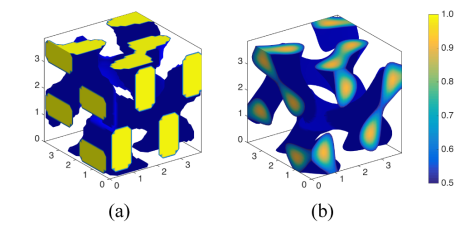
\includegraphics[scale=0.5]{./figures/22.png}
	\caption{gyroid相($I\alpha \bar{3}d$)的三维正视图与(a)水平集法得到的初步猜测和(b)收敛的SCFT解。因为没有涂抹,所以最初的猜测包含了一个有点像素化的界面,它的小特性反映了底层FFT网格的分辨率。计算条件为$\chi N=20,f_A =0.35$,和$b_A/b_B=1$,且网格尺寸为$32\times 32\times 32$。计算得到的结构相对于无序相的每链自由能为$\Delta F /k_b T =-0.63169$。(a)中有争议的结构的尺度维数为4,而由SCFT得到的松弛单元维数为3.85。A块的体积分数是为体积分数$\phi _A(\mathbf{r})\geqslant 0.5$绘制的.
	}
	\label{figure2}
\end{figure}
为了提供一个具体的例子,图\ref{figure22}显示了计算二嵌段共聚物熔体中gyroid相的初始和最终组成剖面。在这种情况下,我们使用了水平集方法,没有模糊的接口,以产生一些什么粗略的初始近似。复制此示例所需的文件在“\href{http://pubs.acs.org/doi/suppl/10.1021/acs.macromol.6b00107/suppl_file/ma6b00107_si_001.pdf}{Supporting Information}”中的文件目录中提供。\\
\textbf{3.4.工作流.}在这一小节中,我们更详细地描述了应用形状因子法生成复杂粒子相的初始猜测的过程。在\href{http://pubs.acs.org/doi/suppl/10.1021/acs.macromol.6b00107/suppl_file/ma6b00107_si_001.pdf}{Supporting Information}部分S6中给出了水平集方法的相应描述。该工作流使用Matlab脚本生成组合轮廓模型,并使用PSCF进行不同场表示之间的转换和求解SCFT方程。
\begin{figure}[H]
	\centering
	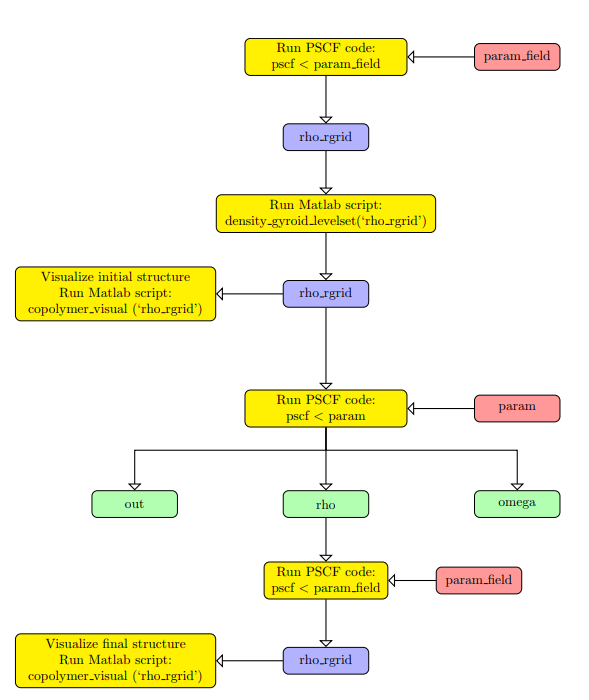
\includegraphics[scale=0.5]{./figures/23.png}
	\caption{流程图描述了使用初始化方法和PSCF代码执行所需的SCFT计算所涉及的步骤。为了开始这个过程,需要将文件(作为\href{http://pubs.acs.org/doi/suppl/10.1021/acs.macromol.6b00107/suppl_file/ma6b00107_si_001.pdf}{Supporting Information}中的存档)density$\_$-phase、Param、param$\_$kgrid和copolymer$\_$visual复制到同一个工作目录中。\href{http://pubs.acs.org/doi/suppl/10.1021/acs.macromol.6b00107/suppl_file/ma6b00107_si_001.pdf}{Supporting Information}部分S1给出了每个文件的描述,\href{http://pubs.acs.org/doi/suppl/10.1021/acs.macromol.6b00107/suppl_file/ma6b00107_si_001.pdf}{Supporting Information}部分S5提供了每个文件的示例,绿色框是聚合SCFT计算的结果,而红色框包含输入文件,黄色框包含用于运行程序的命令行执行语句,蓝色框表示执行计算所需的中间文件或步骤。}
	\label{figure3}
\end{figure}
图\ref{figure23}描述了应用形式因子方法模拟粒子相位的步骤,例如BCC或Frank-kasper$\sigma$相。首先,我们使用Matlab或Octave运行一个名为density$\_$phase的Matlab脚本来计算感兴趣结构的体积分数的Fourier系数。这将输出一个名为rho$\_$kgrid的文件,其中包含使用公式\ref{15}的傅里叶系数。该文件的内容是按照3.1节中的算法创建的。接下来,在名为param$\_$kgrid的参数文件的控制下运行PSCF代码,该文件指示PSCF读取rho$\_$kgrid,应用逆傅里叶变换(使用KGRID$\_$TO$\_$RGRID命令),并输出一个名为rho$\_$rgrid的文件,该文件包含坐标空间网格中所有组件的体积分数的值。然后,可以使用另一个名为copolymer$\_$visual的Matlab脚本可视化rho$\_$rgrid文件,以确认最终猜测的质量正确性,并在必要时调整涂片因子。最后,在一个名为param的参数文件的控制下再次运行PSCF,该文件指示PSCF读取文件rho$\_$rgrid,通过将Lagrange乘子场初始设置为零,从这个体积分数字段模型中生成相应的$\omega$相,然后使用图\ref{figure21}所示的迭代过程,使用该初始猜测求解SCFT方程。如果需要的话,在第一次和第二次调用PSCF期间执行的计算可以合并成一个单独的运行;我们分离它们只是为了让用户有机会在赞成放弃之前可视化rho$\_$rgrid文件,并适当地调整公式\ref{15}中的涂抹因子。当得到一个收敛的溶液时,PSCF将输出两个文件,名为omega和rho,分别包含最终的化学势和体积分数场,第三,一个名为out的文件包含(除其他信息外)每个单体的自由能和有序相的单元尺寸的最终值。\\
\textbf{4.实例研究}

我们通过实验观察到的两个例子证明了形式因子法的适用性:二嵌段共聚物中的离散颗粒相和聚四嵌段共聚物(苯乙烯-b-异戊二烯-b-环氧乙烷)中的核−壳球和圆柱体中的离散颗粒相。\\
\textbf{4.1.二嵌段共聚物中的颗粒形成相。}
双嵌段共聚物在过去已经得到了广泛的研究,目前仍是研究嵌段共聚物相行为的最简单的模型。除了经典例子形成相,如BBC球,最近,在一种聚异戊二烯-丙交酯(IL)二嵌段共聚物中观察到了配合物Frank−Kasper$\sigma$相。$\sigma$相在质量再分布的BBC相中成核,在一个单位细胞内形成五个不同的粒子群。此外,还证明了保持恒定密度的约束$\sigma$相中的“粒子”达到非理想球形的形状。虽然BCC相中的粒子有时被称为球形,但我们将所有这些相称为粒子形成相。

$\sigma$相使用自洽场的研究是一个具有计算挑战性的问题。$\sigma$相有一个巨大的单元,有30个粒子,因此需要大量的网格点来适当地解决这个结构。另一个主要问题是产生一个合理的初始猜测,它能很好地表示结构,足以收敛到SCFT方程的适当解。然而,Xie等人报道了$\sigma$相在SCFT构象不对称二嵌段共聚物中的确定,并预测了它在miktoarm嵌段共聚物中的存在。此外,作者还认为,二嵌段共聚物中两嵌段的统计段长不对称有利于$\sigma$相的形成而不是BCC相的形成。


在本节中,我们演示了我们生成初始势场的方法是通用的,并且可以很容易地应用于复杂的$\sigma$相位。实际上,$\sigma$相所涉及的复杂性是检验该方法的稳健性的理想测试。随后,我们使用同样的方法为另外三个粒子形成阶段(FCC,BCC和A15)生成SCFT解,并在相图中的一个状态点检验所有四个竞争相的相对稳定性。这里,我们只介绍了$\sigma$相阶段的一步的过程,而其他阶段的步骤则在\href{http://pubs.acs.org/doi/suppl/10.1021/acs.macromol.6b00107/suppl_file/ma6b00107_si_001.pdf}{Supporting Information}部分S3中提供。

根据谢氏等人所报道的相图的基础,我们认为AB二嵌段共聚物的熔体体积分数$f_A=0.25$,统计段长的比率是$b_A/b_B=2$,使A嵌段形成粒子,而B填写矩阵。我们首先计算了在公式\ref{15}中给出的域形成粒子的涂抹体积分数剖面。为了评价这个表达式,我们需要以下信息:单元维数来计算reciprocal space vectors $\mathbf{q}$、位置($\mathbf{j}$)和每个粒子的大小(R),并形成粒子的因子振幅$f_j(\mathbf{q})$。在讨论的特定的IL-二嵌段共聚物实验中发现$\sigma$相包含一个a=431A,c=228A四边形单元中。对于四边形单元格,reciprocal空间中的基向量是
\begin{equation}\label{17}
\mathbf{b}_1=\frac{2\pi}{\alpha}\hat{e}_1,~~~\mathbf{b}_2=\frac{2\pi}{\alpha}\hat{e}_2,~~~\mathbf{b}_3=\frac{2\pi}{\alpha}\hat{e}_3
\end{equation}
其中,$\hat{e}_1$、$\hat{e}_2$和$\hat{e}_3$分别是笛卡尔坐标系x、y和z方向上的单位向量。

粒子的位置在实验上是用Wyckoff位置来报告的。利用国际晶体表中P42/MNM空间群的对称运算,将个Wyckoff位置变换为各自的协坐标。例如,4f(0.104,0.104,0)的威望模拟位置导致(0.104 a,0.104 a,0),(0.896a,0.896a,0),(0.396 a,0.604a,0.5c),
以及\\
(0.604a,0.396a,0.396a),0.5C)
作为单元中四个粒子的坐标。“\href{http://pubs.acs.org/doi/suppl/10.1021/acs.macromol.6b00107/suppl_file/ma6b00107_si_001.pdf}{Supporting Information}”第S2节提供了将所有其他Wyckoff位置转换为各自坐标的过程,总共产生了30个粒子。

必须指出的是,粒子在单元格中的确切位置决定了结构的对称性,是一项重要的要求,而粒子的大小和形状可以近似。因此,对于初始化过程,我们假设所有的粒子都是大小相等的球体,并表明这种假设不会妨碍收敛,因为粒子的大小和形状在SCFT迭代过程中会发生调整,但确实会影响收敛速度。用公式\ref{15}计算$\phi _A$所需的球体的形状因子振幅是
\begin{equation}\label{18}
f(\mathbf{q})=\left( \frac{4\pi R^3}{3} \right)F(|\mathbf{q}|R)
\end{equation}
这里
\begin{equation}\label{19}
F(x)=\frac{3\left[ \sin(x) -x\cos(x) \right]}{x^3}
\end{equation}
$\mathbf{q}=(0,0,0)$的值被赋值为$\lim _{x\rightarrow 0} F(X)=1$,给出$f(\mathbf{q}=0)=4\pi R^3/3$。请注意,将此值替换成公式\ref{15},用30个球体代替体积V的单元产生$f(\mathbf{q}=0)=30×(4\pi R^3/3)/V=f_A$,从而得到正确的平均体积分数。这个关系给出了使用等半径的模型的球体半径。B块的体积分数是
\begin{equation}\label{20}
\phi _B(\mathbf{q}) =
\begin{cases}
1-f_A, & \mbox{if }\mathbf{q}=(0,0,0)\\
-\phi _A(\mathbf{q}), & \mbox{if }\mathbf{q}\neq (0,0,0)
\end{cases}
\end{equation}
上述体积分数分布与不可压缩性一致.使用第2.2节描述的索引惯例,必须在$0<m_i<N_i,i=1,2,3$的范围内,计算所有$\mathbf{q}(m_1,m_2,m_3)$的这些Fourier分量。请注意,由于离散周期网格上的值“混叠”,因此在此区域上计算Fourier分量就足够了,因为该区域上只包含$m_1$、$m_2$和$m_3$的非负值,这导致了整数$m_i$与任意方向i的整数乘$N_i$相差无几的波矢的等价性。

我们使用Matlab脚本(在\href{http://pubs.acs.org/doi/suppl/10.1021/acs.macromol.6b00107/suppl_file/ma6b00107_si_001.pdf}{Supporting Information}部分S3.1.1中提供)计算了所有$\mathbf{q}$的少数分量所需的傅里叶振幅,并计算了图\ref{figure23}所示相的对应值。在多次重复涂片系数、$\sigma _{smear}$的情况下,我们选择$\sigma _{smear}=0.35$,即在每个球体中心的体积分数$\phi _A=0.95\pm0.02$。

图\ref{figure24}显示了通过上述计算得到的单元内体积分数剖面的2D和3D视图,这构成了基于实验数据的合理的初始猜测。正如预期的那样,所有的粒子都是大小相等的球体。此外,界面被涂抹和轮廓是光滑的。然后将相应的势场作为初始猜测提供给SCFT迭代器,在$\chi N=25$的中间偏析强度下寻找鞍点。图\ref{figure25}绘制了在收敛的SCFT迭代结束时获得的$\sigma$相的体积分数。计算采用应力松弛的Anderson混合格式。在大约800次迭代中实现了收敛,在一个单独的Intel 2.6GHz处理器上需要12小时。需要指出的是,大部分的计算时间都用于解除单元的应力,这导致了单元尺寸的大约25\%的变化,同时保持了实验报告的比例,$a/c=1.89$。
\begin{figure}[H]
	\centering
	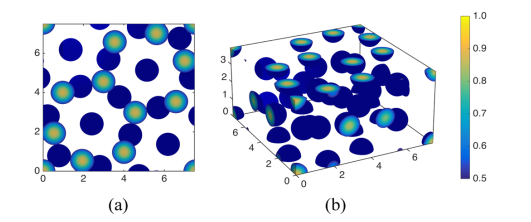
\includegraphics[scale=0.5]{./figures/24.png}
	\caption{(a)二维顶视图和(b)使用上述初始化方法获得的$\sigma$相近似的3D透视视图。为了简化可视化,只绘制体积分数$\phi _A(\mathbf{r})\geq 0.5$的A块的体积分数。涂片系数$\sigma_{smear}=0.2$,被用来得到涂片轮廓。计算的网格尺寸为$128\times 128\times 64$,单元尺寸$a=7.55,c=3.99$。单元的尺寸按未受干扰的根均方端到端长度,$R_{end}=(N_L b_L^2 + N_I b_I 2)^{1/2}$根据实验报告的数值计算,$N_L=13,N_I=47,b_L=9.9A,b_I=6.5A$用于IL二嵌段共聚物。}
	\label{figure4}
\end{figure}

\begin{figure}[H]
	\centering
	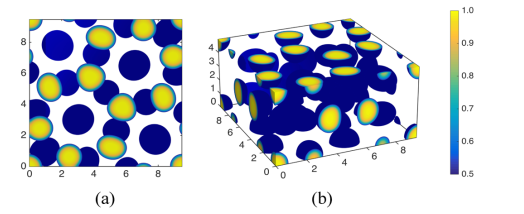
\includegraphics[scale=0.5]{./figures/25.png}
	\caption{(a)二维顶视图和(b)由收敛的SCFT迭代得到的$\sigma$相的三维透视视图。只绘制体积分数$\phi _A(\mathbf{r})\geq 0.5$的A块的体积分数。计算是在$\chi N=25$和$f_A=0.25$的情况下进行的。得到的结构相对于无序相的每链自由能为$\Delta F/k_BT=-0.46950$。应力松弛单元的尺寸$a=9.55,c=5.02$。}
	\label{figure5}
\end{figure}

图\ref{figure24}和图\ref{figure25}的主要区别是单位细胞中粒子的形状和大小发生了显著变化。如图\ref{figure25}所示,在$\sigma$相中有粒子的形状和大小的分布。所得结构的每链自由能相对于无序相的自由能约为$10^{-1}K_BT$与文献报道的计算结果一致。

我们使用同样的方法(\href{http://pubs.acs.org/doi/suppl/10.1021/acs.macromol.6b00107/suppl_file/ma6b00107_si_001.pdf}{Supporting Information}部分S3)生成三个粒子形成阶段的初始势场,这三个阶段应该与$\sigma$相竞争:$BCC,FCC$和$A15$。对于所有情况,涂片轮廓提供给SCFT迭代器。图\ref{figure26}描述了在各自收敛的SCFT迭代结束时获得的所有四个阶段的单元格。请注意,BCC和FCC相仍然有接近球形的粒子,而A15相有扭曲的球体。除A15相和$\sigma$相外,任意两种结构的每链自由能差为$10^{-3}k_BT$,其中差为$10^{-4}k_BT$阶。这突出说明了在比较复杂相时使用SCFT所面临的挑战,因为其结果对统计片段长度和相互作用参数$\chi$的选择极为敏感。我们还注意到,其他三个阶段取得的结果与先前报告的结果是一致的。

我们成功地为复杂的A15和$\sigma$相播种和放松SCFT解决方案,证明了该方法是稳健的。在\href{http://pubs.acs.org/doi/suppl/10.1021/acs.macromol.6b00107/suppl_file/ma6b00107_si_001.pdf}{Supporting Information}部分S3中,我们提供脚本来生成粒子形成阶段的初始势场,这些初始势场可以适当地改变所需的中间阶段,并与PSCF代码一起使用来执行SCFT计算。

\begin{figure}[H]
	\centering
	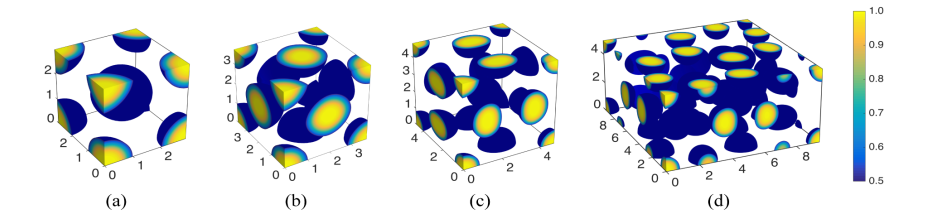
\includegraphics[scale=0.5]{./figures/26.png}
	\caption{(a)BCC,(b)FCC,(c)A15和(d)在各自收敛的SCFT迭代结束时获得的$\sigma$相的3D透视视图。只绘制体积分数$\phi _A(\mathbf{r})\geq 0.5$的A块的体积分数。计算是在$\chi N=25$和$f_A=0.25$的情况下进行的。得到的结构相对于无序相的每链自由能分别为$\Delta F/k_BT=-0.46808,-0.46556,-0.46906,-0.46950$。BCC和FCC的网格尺寸分别为$36\times 36\times 36$,A15和$\sigma$的网格尺寸分别为$64\times 64\times 64$和$128\times 128 \times 64$。}
	\label{figure6}
\end{figure}

所有SCFT计算中的一个问题是选择一个适当的网格大小来平衡精度和计算效率。积分步长$\Delta s$和收敛容差$\epsilon$的选择也会对收敛结果产生影响,但影响程度较小。\href{http://pubs.acs.org/doi/suppl/10.1021/acs.macromol.6b00107/suppl_file/ma6b00107_si_001.pdf}{Supporting Information}部分S9包含关于这些参数对本案例研究的影响的其他信息。\\
\textbf{5.结论}我们提出了两种方法,以产生实际有用的初步猜测,以进行单元SCFT计算所需的势场。为粒子相提出的方法利用以下关于有序微相的信息,对所需的化学势场进行了估计:(1)单元胞的尺寸和类型;(2)形成微结构域的粒子的形状、大小和位置;(3)微观相的空间群对称性。这些信息通常来自散射和电子显微镜实验,这些实验通常用来表征有序的微相。因此,这种方法对于理解实验发现的微相的稳定性和指导实验工作在有前途的方向上具有实用价值。


目前,人们使用Matlab脚本来构造每个感兴趣的结构的组成轮廓的数学模型。开发一个基于计算机辅助设计CAD基的输入也可能是有用的,它可以将用户提供的候选相位的CAD绘图转换为涂抹的化学势场,作为SCFT计算的输入。虽然我们已经提高了基于CPU的PSCF代码处理涉及大单元的问题的能力,但我们也认识到修改代码以使用GPU和/或多个CPU核来加速性能是有用的。

我们通过两个例子论证了我们的方法对粒子相的适用性:二嵌段共聚物中的成球相和在SISO四嵌段三元共聚物的核-壳球和圆柱体。在第一个例子中,我们使用我们的方法生成两个相对简单的相(BCC和FCC)以及复杂的A15和$\sigma$相的势场的猜测值。四个阶段的场的猜测值收敛到各自适当的鞍点,表明该方法是稳健的,只需要台式计算机就可以用于研究嵌段聚合物中的复杂相。此外,我们计算了所有四个相的自由能,并比较了它们在相图中某一特定状态点的相对稳定性。我们还对不同温度值下的无序−BCC和BCC−十六进制跃迁进行了SCFT计算,并与实验结果进行了比较。我们还展示了一个使用水平集方法初始化字段的网络阶段收敛的例子。这里描述的方法是通用的,提供了利用SCFT理解和探索嵌段聚合物中新相的诱人机会。












\end{quotation}
\end{CJK}
\end{document}